\documentclass[12pt]{article}

\usepackage[utf8]{inputenc}
\usepackage[russian]{babel}
\usepackage{geometry}
\usepackage{graphicx}
\usepackage{soul}
\usepackage{color}
\usepackage{colortbl}
\usepackage{multicol}
\usepackage{minted}
\usepackage[all]{xy}	
\geometry{a4paper, top=15mm, bottom=15mm, left=15mm, right=15mm}
\definecolor{emae}{RGB}{132,65,101}

\begin{document}

\setcounter{page}{0}
\thispagestyle{empty}

\begin{center}
    Федеральное государственное автономное учебное учреждение высшего образования\\
    <<Национальный исследовательский университет ИТМО>>\\
\vspace{0.5cm}
    Мегафакультет компьютеных технологий и управления\\
    Факультет программной инженерии и компьютерной техники
\end{center}

\vspace{3cm}

\begin{center}
\Large
\textbf{
    Отчёт\\
    по лабораторной работе №4\\
    <<Исследование протоколов, форматов обмена информацией\\
    и языков разметки документов>>\\
    по дисциплине <<Информатика>>
}
\end{center}

\begin{center}
\large
    Вариант 10
\end{center}

\vspace{6cm}

\begin{flushright}
    Студентка: Богданова Мария Михайловна, группа P3118\\
    Преподаватель: Рыбаков Степан Дмитриевич
\end{flushright}

\vspace{6cm}

\begin{center}
    Санкт-Петербург\\
    2022
\end{center}

\newpage

\tableofcontents

\newpage

\section{Задание}

1. Определить номер варианта как остаток деления на 36 порядкового номера в списке группы в ISU. В случае, если в данный день недели нет занятий, то увеличить номер варианта на восемь.\\
\\
2. Изучить форму Бэкуса--Наура.\\
\\
3. Изучить особенности языков разметки/форматов JSON, YAML, XML.\\
\\
4. Понять устройство страницы с расписанием для своей группы:\\
http://itmo.ru/ru/schedule/0/P3118/schedule.htm\\
\\
5. Исходя из структуры расписания конкретного дня, сформировать файл с расписанием в формате, указанном в задании в качестве исходного. При этом необходимо, чтобы в выбранном дне было не менее двух занятий (можно использовать своё персональное). В случае, если в данный день недели нет таких занятий, то увеличить номер варианта ещё на восемь.\\
\\
6. Обязательное задание (позволяет набрать до 65 процентов от максимального числа баллов БаРС за данную лабораторную): написать программу на языке Python 3.x, которая бы осуществляла парсинг и конвертацию исходного файла в новый. Нельзя использовать готовые библиотеки, в том числе регулярные выражения в Python и библиотеки для загрузки XML--файлов.\\
\\
7. Дополнительное задание №1 (позволяет набрать +10 процентов от максимального числа баллов БаРС за данную лабораторную).\\
\indent a) Найти готовые библиотеки, осуществляющие аналогичный парсинг и конвертацию файлов.\\
\indent b) Переписать исходный код, применив найденные библиотеки. Регулярные выражения также нельзя использовать.\\
\indent c) Сравнить полученные результаты и объяснить их сходство/различие.\\
\\
8. Дополнительное задание №2 (позволяет набрать +10 процентов от максимального числа баллов БаРС за данную лабораторную).\\
\indent a) Переписать исходный код, добавив в него использование регулярных выражений.\\
\indent b) Сравнить полученные результаты и объяснить их сходство/различие.\\
\\
9. Дополнительное задание №3 (позволяет набрать +10 процентов от максимального числа баллов БаРС за данную лабораторную).\\
\indent a) Используя свою исходную программу из обязательного задания, программу из дополнительного задания №1 и программу из дополнительного задания №2, сравнить стократное время выполнения парсинга + конвертации в цикле.\\
\indent b) Проанализировать полученные результаты и объяснить их сходство/различие.\\
\\
10. Дополнительное задание №4 (позволяет набрать +5 процентов от максимального числа баллов БаРС за данную лабораторную).\\
\indent a) Переписать исходную программу, чтобы она осуществляла парсинг и конвертацию исходного файла в любой другой формат (кроме JSON, YAML, XML, HTML): PROTOBUF, TSV, CSV, WML и т. п.\\
\indent b) Проанализировать полученные результаты, объяснить особенности использования формата.\\

\newpage

\section{Ход работы}
\subsection{Обязательное задание}

\begin{footnotesize}
\begin{verbatim}
timetable: 
  day: Вторник 
  lesson1: 
    time: 8:20-9:50 
    room: Акт. зал 
    subject: Информатика (лек) 
    teacher: Балакшин Павел Валерьевич 
    location: ул.Ломоносова, д.9, лит. М 
    format: Очно-дистанционный 
    weeks: 3, 5, 7, 9, 11, 13, 15, 17 
  lesson2: 
    time: 10:00-11:30 
    room: Акт. зал 
    subject: Основы профессиональной деятельности (лек) 
    teacher: Клименков С.В. 
    location: ул.Ломоносова, д.9, лит. М 
    format: Очно-дистанционный 
    weeks: 3, 5, 7, 9, 11, 13, 15, 17 
  lesson3: 
    time: 11:40-13:10 
    room: 1223 
    subject: Программирование (лек) 
    teacher: Письмак А.Е. 
    location: ул.Ломоносова, д.9, лит. М 
    format: Очно-дистанционный 
    weeks: 3, 5, 7, 9, 11, 13, 15, 17 
  lesson4: 
    time: 8:20-9:50 
    room: нет 
    subject: Информатика (лек) 
    teacher: Балакшин Павел Валерьевич 
    location: дома 
    format: Дистанционный 
    weeks: 5 
  lesson5: 
    time: 10:00-11:30 
    room: нет 
    subject: Основы профессиональной деятельности (лек) 
    teacher: Клименков С.В. 
    location: дома 
    format: Дистанционный 
    weeks: 5 
  lesson6: 
    time: 11:40-13:10 
    room: 1223 
    subject: Программирование (лек) 
    teacher: Письмак А.Е. 
    location: дома 
    format: Дистанционный 
    weeks: 5
\end{verbatim}
\end{footnotesize}

\newpage
Код решения основного задания:\\
\inputminted{python}{task1.py}
\newpage

\textbf{Вывод программы - расписание в формате XML:}
\begin{multicols}{2}
\begin{tiny}
\begin{verbatim}
<timetable>
        <day>Вторник </day>
        <lesson1>
            <time>8:20-9:50 </time>
            <place>Акт. зал </room>
            <subject>Информатика (лек) </subject>
            <teacher>Балакшин Павел Валерьевич </teacher>
            <location>ул.Ломоносова, д.9, лит. М </location>
            <format>Очно-дистанционный </format>
            <weeks>3, 5, 7, 9, 11, 13, 15, 17 </weeks>
        </lesson1>
        <lesson2>
            <time>10:00-11:30 </time>
            <place>Акт. зал </place>
            <subject>Основы профессиональной деятельности (лек) </subject>
            <teacher>Клименков С.В. </teacher>
            <location>ул.Ломоносова, д.9, лит. М </location>
            <format>Очно-дистанционный </format>
            <weeks>3, 5, 7, 9, 11, 13, 15, 17 </weeks>
        </lesson2>
        <lesson3>
            <time>11:40-13:10 </time>
            <place>1223 </place>
            <subject>Программирование (лек) </subject>
            <teacher>Письмак А.Е. </teacher>
            <location>ул.Ломоносова, д.9, лит. М </location>
            <format>Очно-дистанционный </format>
            <weeks>3, 5, 7, 9, 11, 13, 15, 17 </weeks>
        </lesson3>
 \end{verbatim}
\end{tiny}       
\columnbreak
\begin{tiny}
\begin{verbatim}        
        <lesson4>
            <time>8:20-9:50 </time>
            <place>нет </place>
            <subject>Информатика (лек) </subject>
            <teacher>Балакшин Павел Валерьевич </teacher>
            <location>дома </location>
            <format>Дистанционный </format>
            <weeks>5 </weeks>
        </lesson4>
            <time>10:00-11:30 </time>
            <place>нет </place>
            <subject>Основы профессиональной деятельности (лек) </subject>
            <teacher>Клименков С.В. </teacher>
            <location>дома </location>
            <format>Дистанционный </format>
            <weeks>5 </weeks>
        </lesson5>
        <lesson6>
            <time>11:40-13:10 </time>
            <place>1223 </place>
            <subject>Программирование (лек) </subject>
            <teacher>Письмак А.Е. </teacher>
            <location>дома </location>
            <format>Дистанционный </format>
            <weeks>5</weeks>
        </lesson6>
</timetable>
\end{verbatim}
\end{tiny}
\end{multicols}

\subsection{Дополнительное задание №1}

Для выполнения этого задания я использовала библиотеки safe\_load и dict2xml. \\
\\Код программы:
\inputminted{python}{task2.py}
Вывод данной программы соответствует выводу программы, реализованной в первом задании, единственное различие можно заметить в последней строке - изменилось время реализации кода  (time:  0.0006699000005028211 -> time:  0.04540479998104274, см. рис 1.)
\newpage
\subsection{Дополнительное задание №2}

При выполнении данного задания я использовала основной код, но некоторые функции в нем заменила регулярными выражениями:
\inputminted{python}{lab4_task3add.py}
\newpage
Содержимое вывода данной программы соответствует содержимому выводов предыдущих программ за исключением времени (time:  0.001284400001168251)
\\
\begin{figure}[h]
    \centering
    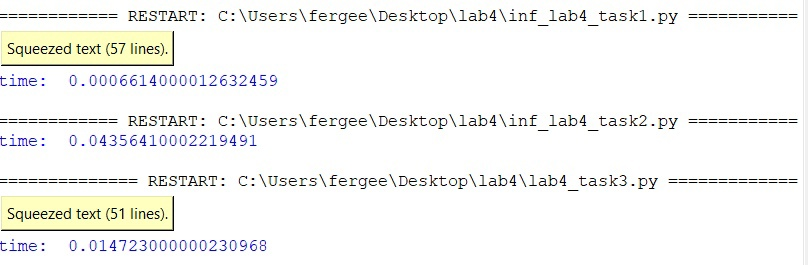
\includegraphics[width=17cm]{ris_1.jpg}
    \caption{Время выполнения всех 3-х программ}
\end{figure}

\subsection{Дополнительное задание №3}

Как я уже упоминала выше, во всех решениях я использовала библиотеку time для того, чтобы засечь время выполнения программ и сравнить их между собой. Я написала цикл, чтобы получить среднее время выполнения.  

\begin{center}
\textbf{	Таблица со сравнением полученных данных:}
\\
\end{center}

\begin{tabular}{|p{11cm}|p{5cm}|}
    \hline
    \centering
    \textbf{Способ} & \textbf{Среднее время выполнения программы}\\
    \hline
    \centering
    \cellcolor{emae}Основное задание (без исп. сторонних библиотек и RE) & \ \ 0.49 с.\\
    \hline
    \centering
    Доп. задание №1 (С исп. библиотек safe\_load и dict2xml) & \ 4.21 с.\\
    \hline
    \centering
    Доп. задание №2 (С исп. RE)  & \ 0.59 с.\\
    \hline
\end{tabular}
\\
\\
\begin{picture}(10,10)
\multiput(10,55)(8,0){40}{\circle*{2}}
\end{picture}
\\
Программа,написанная без использования сторонних библиотек и регулярных выражений, оказалась самой быстрой. Дольше всего работает программа, написанная при выполнении 1-го дополнительного задания, так как она производит рекурсивный парсинг YAML в отличие от двух других программ, в которых происходит отбор по конкретным заданным критериям. Программа с использованием регулярных выражений работает дольше первой, поскольку постоянно происходит проверка данных на соответствие заданному шаблону, однако время выполнение 1-ой и 3-ей программы мало отличается в силу небольшого объема кода. \textbf{Самый быстрый способ выделен в таблице серо-буро-малиновым (в подозрительную крапинку) цветом.}
\\

\begin{figure}[h]
    \centering
    
\includegraphics[width=5cm]{srbk.jpg}
    \caption{светло-серо-буро-малиновый в крапинку цвет}
\end{figure}

\newpage
\section{Вывод}

В ходе выполнения данной лабораторной работы я изучила форму Бэкуса-Наура, особенности языков разметки/форматов JSON, YAML, XML, научилась формировать файлы в этих форматах, писать парсер и конвертировать файлы из одного формата в другой.\\
\\
\begin{huge}
\begin{center}
\LaTeX
\end{center}
\end{huge}
\newpage
\section{Список использованной литературы}

1. Лямин А.В., Череповская Е.Н. Объектно-ориентированное 
программирование. Компьютерный практикум. – СПб: Университет 
ИТМО, 2017. – 143 с. – Режим доступа: https://books.ifmo.ru/ (дата обращения:28.11.2022)\\
2. MSiter - учебник XML [электронный ресурс]. – Режим доступа: https://msiter.ru/ / (дата обращения: 28.11.2022)\\
3. CoderLessons - учебник YAML [электронный ресурс]. – Режим доступа: https://coderlessons.com/ (дата обращения:28.11.2022)\\

\end{document}